
\documentclass[letter,11pt]{article}

% \setlength{\oddsidemargin}{0.25in}  % really 1.5in
% \setlength{\evensidemargin}{0.5in}  % really 1.5in
% \setlength{\textwidth}{6.0in}
% \setlength{\topmargin}{0in}   % really 1in 
% \setlength{\headheight}{0.20in}
% \setlength{\headsep}{0.20in}
% \setlength{\textheight}{8.45in}

\renewcommand{\floatpagefraction}{0.99} 
\usepackage{amstext,graphicx,palatino,listings,bm,setspace,algorithm2e,booktabs,textcomp}
\usepackage{amsmath}
\usepackage{amssymb}
\usepackage[small]{caption}
\usepackage[left=2.54cm,top=2.54cm,right=2.54cm,bottom=0.54cm,nohead,nofoot]{geometry}

\makeatletter
\renewcommand\section{\@startsection{section}{1}{\z@}%
                                {-3.5ex \@plus -1ex \@minus -.2ex}%
                                {2.3ex \@plus.2ex}%
                                {\normalfont\large\bf}}  
\renewcommand\subsection{\@startsection{subsection}{2}{\z@}%
                                {-3.25ex\@plus -1ex \@minus -.2ex}%
                                {1.5ex \@plus .2ex}%
                                {\normalfont\itshape\bf}}
\newcommand{\F}{{$\mathbf{F}$}}   
\renewcommand{\H}{{$\mathbf{H}$}} 
\renewcommand{\P}{{$\phi{x}$}} 
\newcommand{\eg}{{\it e.g. }}
\newcommand{\ie}{{\it i.e. }}

\begin{document}
{\small
\title{\Large{{\bf Investigation of Automated Variance Reduction Techniques for Monte Carlo Shielding Problems}} \\
       \large{{\bf 22.106 Term Project}} }
\author{Jeremy A. Roberts} }
\date{}
\maketitle

%\tableofcontents

\section{Introduction}

The Monte Carlo method is widely believed to be the most accurate method for solving problems in radiation transport.  Unfortunately, due to its very nature---following individual particle histories---certain classes of problems are particularly challenging for the method.  One such class of problems consist of so-called deep penetration shielding problems.  Because the purpose of a shield is to attenuate a particle population by several orders of magnitude, to use the Monte Carlo method requires a sufficient number of histories to ensure that the population, once attenuated, can still provide adequate statistics.  For deep penetration problems, the level of attenuation makes Monte Carlo prohibitively expensive.

To circumvent this issue, several approaches for {\it variance reduction} have been developed over the years.  Variance reduction techniques aim to modify (\ie bias) in some manner the underlying physics in such a way that an {\it unbiased} solution with {\it lower} statistical error is found than an unbiased simulation using the same computational resources.  Haghighat and Wagner \cite{haghighat2003mcv} classify variance reduction techniques in three ways: {\it modified sampling methods} (\eg source biasing, implicit capture), {\it population control methods} (\eg geometry splitting/roulette, weight windows), and {\it semi-analytical methods} (\eg point detectors and DXTRAN).  In this paper, we only analyze methods falling in the first two categories, namely (automated) approaches for source biasing, geometry splitting/roulette, and weight windows.

The rest of this paper is organized as follows.  In Section \ref{sec:tech}, we describe several approaches to variance reduction that use the adjoint or forward fluxes computed via the discrete ordinates method to select parameters for source biasing, geometry splitting, or weight windows. We apply those techniques in Section \ref{sec:results} to some simple slab problems and summarize the impact each technique has on various problem types. Section \ref{sec:conc} provides several concluding remarks.  Finally, Appendix A provides a sample input file based on the problems analyzed in this project, and Appendix B provides a complete listing of the Matlab code.

\section{Automated Variance Reduction Techniques}
\label{sec:tech}

In this section, we describe several automated approaches for variance reduction.  They are ``automated'' in the sense that essentially no user input is required to generate parameters (\eg the user need not define cell importances for geometry splitting).  Throughout, it is assumed that an approximate forward and/or adjoint flux is available, \eg from a discrete ordinates calculation.

\subsection{Geometry Splitting}

Geometry splitting and roulette is a common variance reduction technique that can yield a substantial reduction in computational expense.  The essential idea of geometry splitting is to encourage more particles (of less weight) to fill a region of high importance.  On the other hand, the technique aims to reduce the computational effort of tracking particles in unimportant regions.  Here, we outline the basic algorithm for geometry splitting.

First, the importance of a cell is taken to be the adjoint flux spatially-averaged over a cell.  Note, this implies that a cell importance may still be energy-dependent.  When a particle of weight $w$  exits a cell $A$ with importance $I_A$ and enters a cell $B$ with importance $I_B$ (with $I_A \neq I_B$), two options exist: either $I_B > I_A$ or $I_B < I_A$.  In the first case, the particle is split into a number of particles dependent on the ratio of the importances.  In the latter case, the particle undergoes roulette and is either eliminated or survives with increased weight. Algorithm \ref{alg:geom} provides the basic implementation. 

\begin{algorithm}
 \label{alg:geom}
 \caption{Geometry Splitting and Roulette}
 $r \leftarrow$ $I_B/I_A$ \;
 \eIf{$r > 1$}{
   \eIf{ $\xi < r - \lfloor r \rfloor$}{
     $n$ $\leftarrow$ $\lceil r \rceil$ \;
   }{
     $n$ $\leftarrow$ $\lfloor r \rfloor$ \;
   }
   $w'$ $\leftarrow$ $w/r$ \;
   bank $n-1$ particles and keep following first \;
 }{
   \eIf{$\xi < r $}{
     $w'$ $\leftarrow$ $w/r$ \;
   }{
     kill particle \;
   }
 }
\end{algorithm}

It is worth noting that the algorithm above is  ``expected-value splitting'' which takes $ w' = w/r$ (\ie no rounding) and  chooses $n = \lfloor r \rfloor $ or $ n= \lceil r \rceil$ \cite{booth1985mcv}.  This is in contrast to ``sampled splitting'' which chooses  $n = \lfloor r \rfloor$ or $ n = \lceil r \rceil$ (via sampling) and  defines the weight to be $w'=w/n$ \cite{booth1985mcv}.   Sampled splitting has the benefit of conserving particle weight at each individual split while the expected-value splitting does so only on average.  However, because the sampled splitting approach introduces varying weights at a particular geometry interface, it may adversely affect the variance (whereas the latter approach does not) \cite{haghighat2003mcv}.  Note further that the simplified sampled splitting method given by Brown \cite{brown2005fmc} does not introduce weight fluctuations but does not capture the importance ratio exactly.

\subsection{CADIS}

The Consistent Adjoint-Driven Importance Sampling (CADIS) method was developed by Wagner and Haghighat \cite{wagner1998avr}.  The key idea of CADIS is that the transport biasing (via weight windows) and source biasing are derived in a consistent manner from the adjoint function.  Here, we give an overview of the use of the adjoint in source and transport biasing and how such biasing can be translated into weight window parameters, largely following Wagner and Haghigat \cite{wagner1998avr}.  Note, this development also forms the basic core of the FW-CADIS and pseudo-Cooper methods described below.

\subsubsection{Source Biasing}

We define the response of interest to be
\begin{equation}
 R = \int_P \psi (P) \sigma_d(P)dP \, ,
\end{equation}
where $\psi$ is the forward angular flux, $\sigma_d$ is an objective function (perhaps a flux-to-dose constant), and $P$ represents the spatial-, energy-, and angular-dependent phase space.  Using the well-known adjoint identity
\begin{equation}
 \langle \psi^\dag H \psi \rangle = \langle \psi H^\dag \psi^\dag \rangle \, ,
\end{equation}
where $\psi^\dag$ is the adjoint angular flux, $H^\dag$ is the adjoint transport operator, and  $\langle \rangle$ represents integration over all phase space, it is possible to show that 
\begin{equation}
 R = \int_P \psi^\dag (P) q(P)dP \, ,
\end{equation}
where $q$ is a forward source density.  Hence, we find that $\psi^\dag$ can be interpreted physically as the expected contribution of a particle anywhere in phase space to the response of interest (\ie the particle importance).

We can use this notion of $\psi^\dag$ to bias the source density $q$ via
\begin{equation}
 \hat{q} = \frac{\psi^\dag(P) q(P) }{ \int_P \psi^\dag(P) q(P) dP } \, ,
 \label{eq:biassrc}
\end{equation}
which can be shown to minimize the variance for $R$.  The particle weights are then defined to be
\begin{equation}
 w(P) = \frac{R}{\psi^\dag(P)} \, .
\end{equation}

\subsubsection{Transport Biasing}
 To investigate transport biasing, consider the integral form of the transport equation,
\begin{equation}
 \psi(P) = \int f(P'\to P) \psi(P') dP' + q(P) \, ,
\end{equation}
where $f(P' \to P) dP$ is the expected number of particles entering $dP$ about $P$ due to an interaction in $P'$, and $q(P)$ is the (forward) source density.  We define
\begin{equation}
 \hat{\psi}(P) = \frac{ \psi^\dag(P)\psi(P) }{ \int \psi^\dag(P)\psi(P) dP } \, ,
 \label{eq:contflux}
\end{equation}
from which we find a transformed integral equation in terms of the biased source:
\begin{equation}
\begin{split}
 \hat{\psi}(P) &= \int dP' f(P'\to P) \frac{ \psi(P')\psi^\dag(P) }{ \int \psi^\dag(P)\psi(P) dP} + \hat{q}(P) \\
               &= \int dP' f(P'\to P) \frac{ \psi(P')\psi^\dag(P) }{ \int \psi^\dag(P)\psi(P) dP}  \frac{ \hat{\psi}(P') \int \psi^\dag(P')\psi(P') dP}{\psi^\dag(P')\psi(P') }+ \hat{q}(P) \\
               &= \int dP' f(P'\to P) \frac{ \psi^\dag(P) \hat{\psi}(P') }{\psi^\dag(P') }+ \hat{q}(P) \, .
\end{split}
\label{eq:modeq}
\end{equation}
In more compact form, we have
\begin{equation}
  \hat{\psi}(P) = \int \hat{f}(P' \to P) \hat{\psi}(P') dP' + \hat{q}(P) \, ,
\end{equation}
where \footnote{It is interesting to note that the modified flux $\hat{\psi}$ in Eq. \ref{eq:contflux} is just the normalized ``contributon flux'' and $\hat{f}$ of Eq. \ref{eq:modf} is akin to the ``contributon cross-section'' (see \eg the interesting paper by M. Williams \cite{williams1991gcr}).  With these interpretations, one can arrive (in hand-waving fashion) to the notion of zero variance.  Since ''contributons'' represent exactly a flow of response from the source to the detector, their very existence gives use what we want; of course, that requires both a perfect knowledge of the adjoint and a way to use it completely.  Unfortunately, we have neither.}
\begin{equation}
 \hat{f}(P' \to P) = f(P' \to P) \frac{\psi^\dag(P) }{\psi^\dag(P') } \, .
 \label{eq:modf}
\end{equation}
Here, $\hat{f}$ represents a biased transfer function that acts to bias the transport process, and $\hat{\psi}$ is the corresponding solution (essentially a contributon flux, a quantity with a very definite physical interpretation that the authors never quite point out; see the note below).  

In general $f(P'\to P)$ is not known, so the modified transport Eqs. \ref{eq:modeq} and \ref{eq:modf} cannot be solved.  However, Eq. \ref{eq:modf} in particular suggests a possible way to modify the population of particles propagating through phase space.  If a particle in phase space $P'$ enters a region in phase space $P$ which is more (less) important than $P'$, then particles can be split (rouletted) based on the value of $\psi^\dag (P) / \psi^\dag (P')$.  This is exactly the idea used in geometry splitting above, but for geometry splitting, the ratio of adjoints is determined only at cell boundaries and not after every interaction in phase space.  After splitting/rouletting, the particle weights are defined via
\begin{equation}
 w(P) = w(P') \frac{\psi^\dag(P')}{\psi^\dag(P)} \, .
\end{equation}

\subsubsection{Implementation}
To implement CADIS, we follow the approach of Wagner and Haghighat in their implementation of CADIS in MCNP \cite{wagner1998avr}.  Because storing adjoint information for all (discretized) phase space can be very expensive for large problems, the angular variable is integrated out of all the quantities of the previous sections.  Consequently, our biased source density becomes
\begin{equation}
 \hat{q}(r,E) = \frac{\phi^\dag(r,E) q(r,E) }{ \int_E \int_V \phi^\dag(r,E) q(r,E) dr dE } \, ,
 \label{eq:biassrc2}
\end{equation}
where $\phi^\dag(r,E)$ is the adjoint scalar flux, and the particle weights are defined as
\begin{equation}
 w(r,E) = \frac{R}{\phi^\dag(r,E)} \, .
\end{equation}

For transport biasing, the weight window approach is used.  The goal of weight-windows is not only to encourage a large number of particles toward a desired region of phase space but to ensure the particles have weights distributed in a relatively narrow range.  A low variance in the weights of particles reaching a detector corresponds directly to a detector response with low variance.  Whenever a particle of weight $w$ enters a region of phase space with a weight window defined by a lower weight $w_L$ and upper weight $w_U$, three possibilities exist.  First, if $w$ is within the weight window, then nothing occurs.  If instead $w < w_L$, a game of roulette is played.  Finally, if $w > w_L$, then the particle is split. Algorithm \ref{alg:ww} outlines a basic weight-window approach modified from \cite{brown2005fmc}.

\begin{algorithm}
 \caption{Weight Windows}
    Input: $w_L(E)$ for each spatial cell and $c_U$ such that $w_U = w_L/c_U$ \;
    \uIf{$w > w_U$ }{
      $n = \lfloor 1+ w/w_U \rfloor$ \;
      \If{$ n > 1 $}{
	$w'$ $\leftarrow$ $w/n$ \;
	bank $n-1$ particles and keep following first \;
      }
    }{
    \uElseIf{$w < w_L $}{
      $P \leftarrow 2w/(w_U+w_L)$ \;
      \eIf{$\xi < P $}{
	$w'$ $\leftarrow$ $w/P$ \;
      }{
	kill particle \;
      }
     }{
     \Else{
       particle is within the weight window
     }
     }
     }
 \label{alg:ww}
\end{algorithm}

Note, it is possible to limit the split ratio, but we choose not to do that since it would reduce the accuracy with which the underlying adjoint (to be used to define $w_L$) is used to bias the transport.  Moreover, $P$ could also be defined differently.  Brown defines a general $P = w/w_{\mathrm{avg}}$ where $w_{\mathrm{avg}}$ is the average weight of the particle if it survives roulette; here, we take that simply to be in the center of the weight window.  %Finally, note that even if $w/w_U > 1$, splitting may not occur.  We conserve weight and avoid varied weight, but miss out on a bit of the underlying adjoint information.  

In using the adjoint to define the weight window bounds, we would like the underlying statistical weight of the particles in $(r,E)$ to be in the center of the bounds.  For a weight window width $c_U = w_U/w_L$, we obtain our goal by defining
\begin{equation}
\begin{split}
  \frac{R}{\phi^\dag(r,E)} &= \frac{1}{2}(w_L + w_U) \\
                           &= \frac{1}{2}(w_L + c_U w_L) \\
                           &= w_L \frac{1+c_U}{2}\, ,
\end{split}
\end{equation}
or 
\begin{equation}
 w_L(r,E) = \frac{R}{\phi^\dag(r,E)} \frac{2}{1+c_U} \, .
\end{equation}
Because the source is biased such that particles born at $(r,E)$ have weight $R/\phi^\dag(r,E)$, the source particles are automatically born within their local weight window.  For some problems, this is very significant.  For example, suppose the response of interest were a small detector on the outside of a reactor vessel.  Then the associated adjoint is bound to vary by orders of magnitude throughout the source region, that is the reactor core.  If the source were not biased consistently with the weight windows, then a particle born could immediately have to undergo splitting or rouletting, thus needlessly wasting computational effort.

\subsection{FW-CADIS}

Forward-Weighted CADIS (FW-CADIS) is a modification of the CADIS method recently developed at Oak Ridge National Laboratory (ORNL) \cite{peplow2009sot,wagner2009fwc}.  Many studies have shown that CADIS performs remarkably well for source-detector problems.  However, it does not do as well for problems with several detectors or more general ``global'' problems.

As a result, FW-CADIS was developed.  The basic motivation of FW-CADIS is to generate a more uniform Monte Carlo particle population across the regions of interest or perhaps over the whole problem domain.  Doing so, it has been suggested, leads to (nearly) uniform statistical uncertainties \cite{cooper2001aww}.  Hence, while uniform Monte Carlo particle density is not really a ``physical'' response, it is nonetheless an attractive goal.  The objective then becomes to find an adjoint function that represents the importance of particles to this response.

Following Wagner et al \cite{wagner2009fwc}, we cast the problem (\ie finding uniform Monte Carlo particle density) into the familiar response formulation
\begin{equation}
 R = \int \psi(P) f(P) dP \, ,
\end{equation}
where again $P$ represents all phase space and $f(P)$ converts physical flux to the Monte Carlo particle density.  The physical particle density $n(P)$ is related to the the Monte Carlo particle density $m(P)$ via
\begin{equation}
 n(P) = \bar{w}(P)m(P) \, ,
\end{equation}
where $\bar{w}(w)$ is the average statistical weight at $P$. Since $\psi(P) = n(P)v(P)$, where $v$ is the velocity, we find that
\begin{equation}
 m(P) = \frac{n(P)}{\bar{w}(P)} = \frac{\psi(P)}{\bar{w}(P)v(P)} = \psi(P) f(P) \, .
\end{equation}
Hence, we may rewrite the total response
\begin{equation}
 R = \int \frac{\psi(P)}{\bar{w}(P)v(P)} dP \, .
\end{equation}
Now if we want the Monte Carlo particle density to be constant,  then $m\propto constant$, and consequently $\bar{w} \propto n$ or equivalently, $\bar{w} v \propto \psi$.  Hence, we may substitute $\bar{w} v = \psi$ into the response equation:
\begin{equation}
 R = \int \psi(P) \frac{1}{\psi(P)} dP \, ,
\end{equation}
which suggests that the adjoint source should be defined as
\begin{equation}
 q^\dag(P) = \frac{1}{\psi(P)} \, .
\end{equation}

This approach can be generalized for any desired response, say a reaction rate with cross-section $\sigma_r(r,E)$ in a specific volume $V$, by defining the adjoint source to be
\begin{equation}
q^\dag(r,E) = 
\begin{cases} \frac{\sigma_r(r,E)}{ \int_E \sigma_r(r,E) dE} &  r\in V \\
              0 &  r \notin V \\
\end{cases} \, .
\end{equation}
With the adjoint source defined for the a particular desired response, the adjoint flux is computed and the CADIS method is used as described above.

\subsection{Pseudo-Cooper's Method}
In contrast to the adjoint-based methods described above, Cooper and Larsen have suggested a different approach to weight window generation based solely on the (inverted) forward flux \cite{cooper2001aww}.  Their method as described in the original paper is actually quite complicated. Nonetheless, the basic idea is clear: ``[I]f the center of the weight window in each cell is chosen to be proportional to the density of physical particles in the cell, then the density of Monte Carlo particles throughout the system is approximately constant'' \cite{cooper2001aww}.  

In fact, this might have been surmised above when we went from $m = constant$ to $\bar{w}v=\psi$; instead of trying to define an adjoint source, we can simply enforce the weight window centers to coincide with an approximate forward flux.   Noting that we previously had set $w = R/\phi^\dag$ and we now want $w \propto \phi$, we conclude that within the adjoint-based framework above, we are now simply setting $\phi^\dag = 1/\phi$.

Instead of implementing Cooper's method exactly (which involves Monte Carlo updates of the weight window parameters via use of Eddington factors and the quasi-diffusion method), we simply use the the inverse forward scalar flux $1/\phi$ in place of the adjoint scalar flux $\phi^\dag$ in the weight window framework described above, \ie a pseudo-Cooper's method.  Consequently, the lower weight window bounds become
\begin{equation}
 w_L(r,E) = \frac{2R\phi(r,E)}{1+c_U} \, ,
\end{equation}
with corresponding particle weights of
\begin{equation}
 w(r,E) = R\phi(r,E) \, .
\end{equation}

One might notice an apparent contradiction: both FW-CADIS and Cooper's method aim to achieve a constant Monte Carlo particle population (and as will be seen below, Cooper's method fairs better for the sample problems investigated).  However, E. Larsen has stated that no zero-variance method exists (at least currently) for global $\psi$ estimates \cite{larsen2007hmc}.  Hence, though FW-CADIS appears to be using a sound adjoint-based formalism, such a formalism was developed for a source-detector problem, where the response $R$ was of interest---not the flux itself.  Consequently, neither FW-CADIS nor Cooper's method actually intend (in some limit) to provide a globally zero variance flux; they in some sense are more heuristic.  While for the simple problems below, the pseudo-Cooper approach wins, work at ORNL suggests Cooper's method does not do as well as FW-CADIS for real-world problems \cite{wagner2009fwc}.

\section{Results}
\label{sec:results}
In this section, we aim to apply the methods of Section \ref{sec:tech} to some simple slab problems.  For this purpose, a one-dimensional multi-group Monte Carlo code was written.  The code treats a finite slab as a number of user-specified coarse meshes within which material properties are constant.  The flux is estimated in each coarse mesh via both the track length and collision density estimators.  Only isotropic scattering in the lab system is treated.

Each of the variance reduction schemes described above is implemented in addition to implicit capture.  For the forward and adjoint scalar flux estimates, a one-dimensional discrete ordinates code was written.  The spatial meshing stems from the slab coarse meshes, and the user additionally specifies the number of fine meshes within each coarse mesh.  Again, materials are constant within a coarse mesh.  Note, the code handles only vacuum boundaries, downscattering, and isotropic scattering in the lab system.  The Gauss-Legendre quadrature scheme for 2, 4, 8, 16, and 32 ordinates is currently implemented following Lewis and Miller \cite{lewis1993cmn}.  However, for all the primary problems, an order of 32 was used (with 10 fine meshes per region).  The final problem revisits a source-detector problem and the effect of $S_N$ order on speed-up.

\subsection{1-Group Source-Detector}

The first problem is a simple monoenergetic source-detector problem.  The slab is 10 cm wide and divided into 20 equally sized coarse meshes.  A uniform isotropic source is located in the first coarse mesh, and the region of interest is the last coarse mesh.  The response of interest is simply the flux.  The material properties are: $\Sigma_T = 1.5$, $\Sigma_a = 0.5$, and $\Sigma_s = 1.0$, all in 1/cm.  Figure \ref{fig:diagram_of_slab} provides a schematic where $S$ denotes the source, and $D_f$ corresponds the ``far detector'' of interest here.

\begin{figure}[h] 
   \centering
   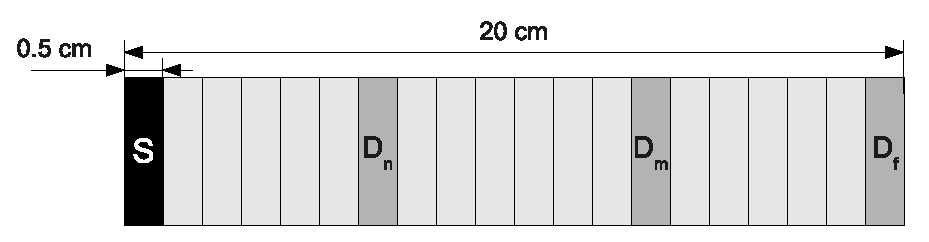
\includegraphics[keepaspectratio, width = 5.0 in]{diagram_of_slab}
   \caption{Basic schematic of one-dimensional slab.}
   \label{fig:diagram_of_slab}
\end{figure}

This problem was solved using analog Monte Carlo, implicit capture, geometry splitting, CADIS, and pseudo-Cooper's method.  Table \ref{tbl:1gsd} provides for each method the figure-of-merit (FOM) for the track length flux estimate, the speed-up relative to analog, and the extrapolated time to 1\% relative error.  To compute the extrapolated time, it is assumed that $RE \propto \sqrt{N} \propto \sqrt{t}$, which is generally valid assuming sufficient sampling.  An $S_N$ order of 32 was used, with ten fine meshes per coarse mesh.

\begin{table}[th]
 \caption{Comparison of methods for one-dimensional, one group source-detector problem.}
 \begin{center} 
 {\small
 \begin{tabular*}{0.99\textwidth}{@{\extracolsep{\fill}} rcccccc } 
  \toprule 
   {\sc METHOD}  &  $\phi$ [n/cm$^2$]  &  {\sc RE} & {\sc FOM} &  {\sc Speed-Up} & {\sc T [s]} & {\sc T$_{\mathrm{1\% RE}}$ [hr]} \\
  \midrule 
   analog      & 3.07E-06 & 0.3612 & 3.48E-03 & 1.00E+00 & 2.20E+03 & 797.62 \\
   imp. capt.  & 3.12E-06 & 0.1141 & 1.75E-02 & 5.03E+00 & 4.39E+03 & 158.59 \\
   geom. sp.   & 3.25E-06 & 0.0036 & 1.11E+01 & 3.18E+03 & 6.91E+03 & 0.25 \\
   CADIS       & 3.25E-06 & 0.0036 & 1.10E+01 & 3.16E+03 & 6.96E+03 & 0.25 \\ 
   Cooper      & 3.24E-06 & 0.0033 & 1.12E+01 & 3.21E+03 & 8.40E+03 & 0.25 \\
  \bottomrule 
 \end{tabular*} 
 }
 \end{center} 
 \label{tbl:1gsd}  
\end{table}

From Table \ref{tbl:1gsd}, it is apparent that analog Monte Carlo for this problem is impractical if we require 1\% RE---nearly 800 hours would be needed.  Implicit capture is seen to reduce this by roughly a factor of five.  However, geometry splitting, CADIS, and pseudo-Cooper give far better speed ups of roughly 3000 (and reduce the time to 1\% RE to less than one half-hour).  While pseudo-Cooper gives the best FOM, since this is such a simple problem, it is difficult to say which of the three automated methods is best, since their FOM's are all very similar.


\subsection{1-Group, Multiple Detectors}

For the same problem configuration depicted in Figure \ref{tbl:1gsd}, we are now interested in three tallies: a near detector $D_n$, a middle detector $D_m$, and the (same) far detector $D_f$.  Table \ref{tbl:1g3d} provides the flux (track length), relative error, FOM, speed up, and time to 1\% relative error of each method for each detector.

For the near detector, the FOM's of all the methods are between 20 and 40, except for the CADIS with an adjoint in the near detector only and CADIS with an adjoint source uniformly distributed between the three detectors.  This makes sense: little speedup is needed or expected from the methods that place an adjoint far past the detector.  The two CADIS example have a large adjoint at the detector, and so its response---the flux---is optimized.

For the middle and far detectors, however, the analog and implicit capture cases do quite poorly.   Geometry splitting (with the adjoint only at the far detector; adjoint placed in near detectors led to excessive splitting) performs pretty well.  CADIS is seen to fail at those detectors if the adjoint is included at previous detectors, \eg the far detector fails if the adjoint is placed at the middle detector.  The CADIS case in which an adjoint source is placed at all three detectors is a powerful example of why simply spreading an adjoint source uniformly across equally important responses is not efficient in practice.  The reason is likely as follows.  The weight windows do a good job of getting many particles to the first detector.  Thereafter, particles encounter a steep drop in the importance of regions and likely suffer significant rouletting.  When they get closer to the second detector, the importance rises sharply again, and hence the particles are split, and so on.  The process has an inherent inefficiency; even if the adjoint information is essentially perfect for those later detectors, all the splitting and rouletting needed to approximate its biasing effect is highly inefficient.  

On the other hand, FW-CADIS does a nice job of spreading the variance.  While the individual CADIS cases do better than the FW-CADIS case, the FW-CADIS ``optimizes'' all three responses better than any single CADIS case.  For example, the ratios of FW-CADIS speed-ups to the far CADIS case speed-ups are 1.34, 1.15, and 0.89, respectively.  While the total computation time in this case is highly dominated by the far detector, and so the benefit of FW-CADIS to the nearer detectors is of little consequence, one can imagine a three-dimensional problem for which a single FW-CADIS could outperform individual CADIS runs.  Pseudo-Cooper slightly outperforms the far CADIS case, but the ratio of its speed-ups to the far CADIS speed-ups for the nearer detectors is below unity; in effect, pseudo-Cooper spends more time on particles in the low-flux region.


\begin{table}[!]
 \caption{Comparison of methods for one-dimensional, one group source-detector problem.}
 \begin{center} 
 \small{
 \begin{tabular*}{0.90\textwidth}{@{\extracolsep{\fill}} rccccc } 
  \toprule 
   {\sc METHOD}  &  $\phi$ [n/cm$^2$]  &  {\sc RE} & {\sc FOM} &  {\sc Speed-Up} & {\sc T$_{\mathrm{1\% RE}}$ [s]} \\
  \midrule 
   {\sc near}   &  & & & &  \\
  \midrule
   analog      & 1.71E-02 & 4.34E-03 & 2.41E+01 & 1.00E+00 & 4.14E+02 \\
   imp. capt.  & 1.70E-02 & 2.40E-03 & 3.96E+01 & 1.64E+00 & 2.53E+02 \\
   geom. sp.   & 1.69E-02 & 1.32E-02 & 3.14E+01 & 1.30E+00 & 3.18E+02 \\
   CADIS (n)   & 1.69E-02 & 1.26E-02 & 7.21E+01 & 2.99E+00 & 1.39E+02 \\
   CADIS (m)   & 1.69E-02 & 1.31E-02 & 4.17E+01 & 1.73E+00 & 2.40E+02 \\
   CADIS (f)   & 1.69E-02 & 2.10E-03 & 3.34E+01 & 1.38E+00 & 3.00E+02 \\
   CADIS (3)   & 1.69E-02 & 2.00E-03 & 7.31E+01 & 3.03E+00 & 1.37E+02 \\
   FW-CADIS    & 1.69E-02 & 4.09E-03 & 4.48E+01 & 1.86E+00 & 2.23E+02 \\
   Cooper      & 1.70E-02 & 2.00E-03 & 3.00E+01 & 1.24E+00 & 3.33E+02 \\
  \midrule 
   {\sc middle}   &  & & & & \\
  \midrule
   analog      & 1.71E-04 & 4.37E-02 & 2.38E-01 & 1.00E+00 & 4.21E+04 \\
   imp. capt.  & 1.79E-04 & 1.86E-02 & 6.59E-01 & 2.77E+00 & 1.52E+04 \\
   geom. sp.   & 1.77E-04 & 1.93E-02 & 1.47E+01 & 6.16E+01 & 6.82E+02 \\
   CADIS (n)   & 1.59E-04 & 3.32E-01 & 1.04E-01 & 4.37E-01 & 9.62E+04 \\
   CADIS (m)   & 1.75E-04 & 1.85E-02 & 2.08E+01 & 8.75E+01 & 4.80E+02 \\
   CADIS (f)   & 1.79E-04 & 3.00E-03 & 1.58E+01 & 6.64E+01 & 6.33E+02 \\
   CADIS (3)   & 1.77E-04 & 1.24E-02 & 1.88E+00 & 7.90E+00 & 5.32E+03 \\
   FW-CADIS    & 1.78E-04 & 6.43E-03 & 1.81E+01 & 7.61E+01 & 5.53E+02 \\
   Cooper      & 1.78E-04 & 2.70E-03 & 1.58E+01 & 6.64E+01 & 6.34E+02 \\
  \midrule 
   {\sc far}   &  & & & & \\
  \midrule
   analog      & 3.07E-06 & 3.61E-01 & 3.48E-03 & 1.00E+00 & 2.87E+06 \\
   imp. capt.  & 3.12E-06 & 1.14E-01 & 1.75E-02 & 5.03E+00 & 5.71E+05 \\
   geom. sp.   & 3.25E-06 & 3.60E-03 & 1.11E+01 & 3.18E+03 & 9.02E+02 \\
   CADIS (n)   &      n/a &      n/a &      n/a &      n/a &  n/a     \\
   CADIS (m)   & 3.98E-06 & 2.44E-01 & 1.20E-01 & 3.45E+01 & 8.31E+04 \\
   CADIS (f)   & 3.25E-06 & 3.61E-03 & 1.10E+01 & 3.16E+03 & 9.09E+02 \\
   CADIS (3)   & 3.59E-06 & 9.08E-02 & 3.53E-02 & 1.01E+01 & 2.83E+05 \\
   FW-CADIS    & 3.25E-06 & 8.74E-03 & 9.79E+00 & 2.81E+03 & 1.02E+03 \\
   Cooper      & 3.24E-06 & 3.30E-03 & 1.12E+01 & 3.21E+03 & 8.96E+02 \\
  \bottomrule 
 \end{tabular*} 
 }
 \end{center} 
 \label{tbl:1g3d}  
\end{table}


\subsection{1-Group, Globally Uniform Statistics}

It may sometimes be the case that low statistical uncertainty is required everywhere in a problem.  Here, we investigate the same slab but employ methods to yield  uniform statistical uncertainties throughout.  Specifically, the FW-CADIS and pseudo-Cooper method were used.  For the former, a uniform adjoint source across the slab was used.  The relative statistical error in each coarse mesh is shown in Figure \ref{fig:1gstat} for FW-CADIS, pseudo-Cooper, and CADIS with an adjoint source in the far detector.  Additionally, Figure \ref{fig:1gmcps} shows the Monte Carlo particle density (using a collision estimator) for each method.  

From Figure \ref{fig:1gstat}, it is apparent that pseudo-Cooper does the best to minimize the uncertainty in deeper regions.  CADIS yields only slightly higher uncertainties.  Surprisingly, FW-CADIS does worse than the others.  This is further exemplified by the steadily decreasing Monte Carlo particle density for FW-CADIS in \ref{fig:1gmcps}, whereas pseudo-Cooper maintains a relatively high constant density and CADIS a slightly lower constant density.

\begin{figure}[h] 
   \centering
   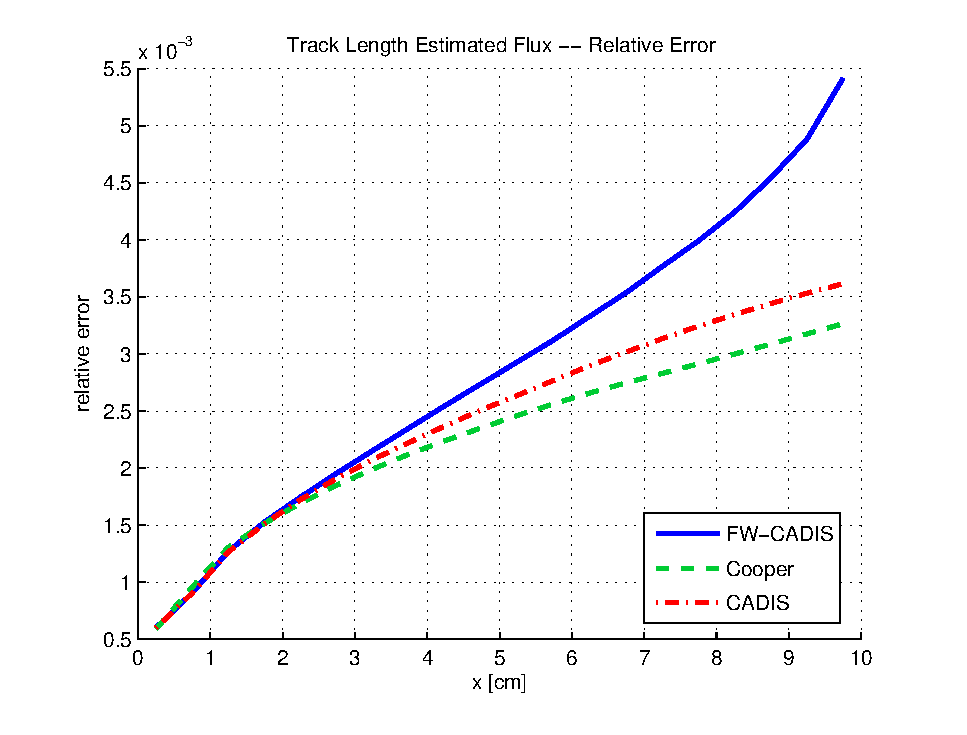
\includegraphics[keepaspectratio, width = 4.0 in]{1gstat}
   \caption{Relative statistical error throughout slab.}
   \label{fig:1gstat}
\end{figure}

\begin{figure}[h] 
   \centering
   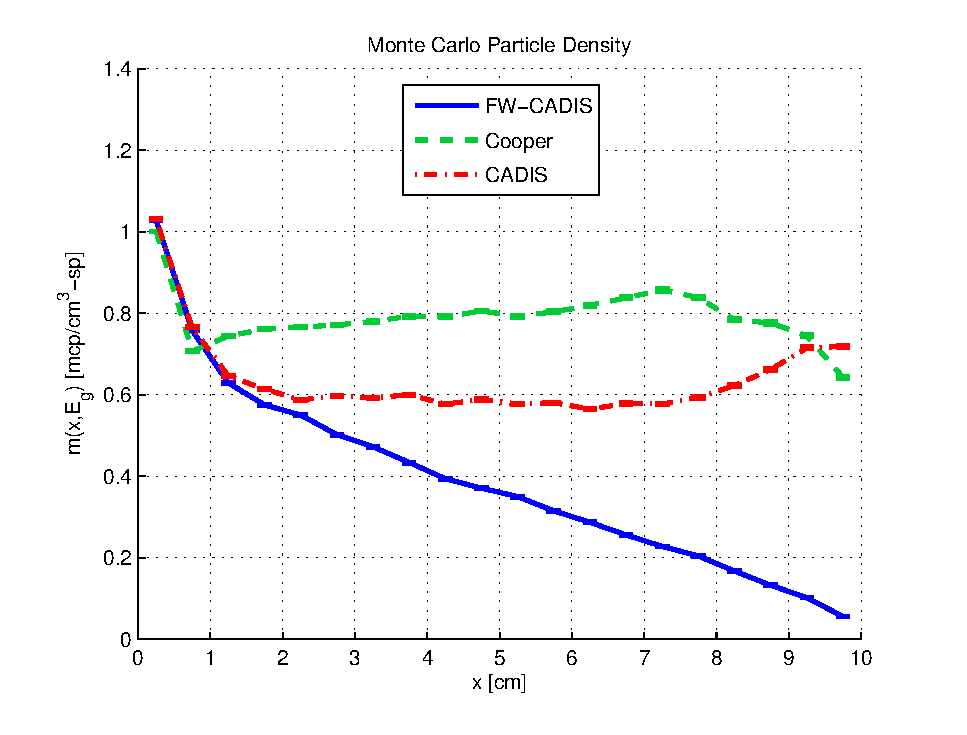
\includegraphics[keepaspectratio, width = 4.0 in]{1gmcps}
   \caption{Monte Carlo particle density throughout slab.}
   \label{fig:1gmcps}
\end{figure}


\subsection{3-Group Source-Detector}

This problem is a three group variation of the source detector problem. Now, the source is uniform, isotropic, and in the first (fast) group.  The detector of interest is the third group (thermal) flux in the far detector.  The slab is again homogeneous with the properties listed in Table \ref{tbl:3groupdata}.

\begin{table}[th]
 \caption{Three group macroscopic cross-sections (in 1/cm).}
 \begin{center} 
 {\small
 \begin{tabular*}{0.60\textwidth}{@{\extracolsep{\fill}} cccccc} 
  \toprule 
    & $\Sigma_t$ & $\Sigma_a$ & $\Sigma_{sg\to1}$ & $\Sigma_{sg\to2}$ & $\Sigma_{sg\to3}$  \\
  \midrule 
   group 1 & 1.0 & 0.2 & 0.3 & 0.2 & 0.2 \\ 
   group 2 & 1.5 & 0.9 & 0.0 & 0.4 & 0.2 \\ 
   group 3 & 2.0 & 0.5 & 0.0 & 0.0 & 1.5 \\ 
  \bottomrule 
 \end{tabular*}
 } 
 \end{center} 
 \label{tbl:3groupdata}  
\end{table}

From Table \ref{tbl:3gsd}, first note that the analog time to 1\%RE is significantly less than the one group problem.  This is because the detector is thermal, and neutrons tend to moderate as they move through the slab.  Furthermore, for this problem implicit capture actually underperforms the analog case.  Both geometry splitting and CADIS provide speed-ups of nearly 500, whereas pseudo-Cooper achieves just half of that.  This is because pseudo-Cooper propagates neutrons of {\it all} groups through the domain, and hence wastes some effort transporting particles that do not contribute to the detector.

\begin{table}[th]
 \caption{Comparison of methods for three group source-detector problem.}
 \begin{center} 
{\small
 \begin{tabular*}{0.90\textwidth}{@{\extracolsep{\fill}} rcccccc } 
  \toprule 
   {\sc METHOD}  &  $\phi$ [n/cm$^2$]  &  {\sc RE} & {\sc FOM} &  {\sc Speed-Up} & {\sc T [s]} & {\sc T$_{\mathrm{1\% RE}}$ [hr]} \\
  \midrule 
   analog      & 1.25E-05 & 0.0695 & 1.66E-02 & 1.00E+00 & 1.25E+04 & 167.55 \\
   imp. capt.  & 1.31E-05 & 0.1248 & 1.09E-02 & 6.58E-01 & 5.89E+03 & 254.62 \\
   geom. sp.   & 1.21E-05 & 0.0091 & 7.70E+00 & 4.64E+02 & 1.58E+03 &  0.36 \\
   CADIS       & 1.22E-05 & 0.0090 & 7.87E+00 & 4.75E+02 & 1.58E+03 & 0.35 \\ 
   Cooper      & 1.21E-05 & 0.0064 & 4.37E+00 & 2.64E+02 & 5.57E+03 & 0.63 \\
  \bottomrule 
 \end{tabular*} 
}
 \end{center} 
 \label{tbl:3gsd}  
\end{table}



\subsection{3-Group, Globally Uniform Statistics}

Here, the same global problem as above is performed using three groups.  For FW-CADIS, a uniform adjoint source in group 3 is used, and for CADIS, a group 3 far detector is used.  Figure \ref{fig:3gstat} shows the relative uncertainties, and Figure \ref{fig:3gmcps} shows the Monte Carlo particle density.  

Evidently, pseudo-Cooper yields the lowest uncertainties for most of the slab.  FW-CADIS gives a steadily increasing uncertainty, as in the one-group problem.  The CADIS uncertainties essentially follow what is expected for a thermal detector: the fast group uncertainty rises in uncertainty, while the thermal group uncertainty falls.  

From Figure \ref{fig:3gmcps}, pseudo-Cooper gives by far the most uniform densities (across all groups).  FW-CADIS provides a relatively flat thermal distribution, and CADIS yields a significantly growing thermal distribution.

\begin{figure}[!] 
   \centering
   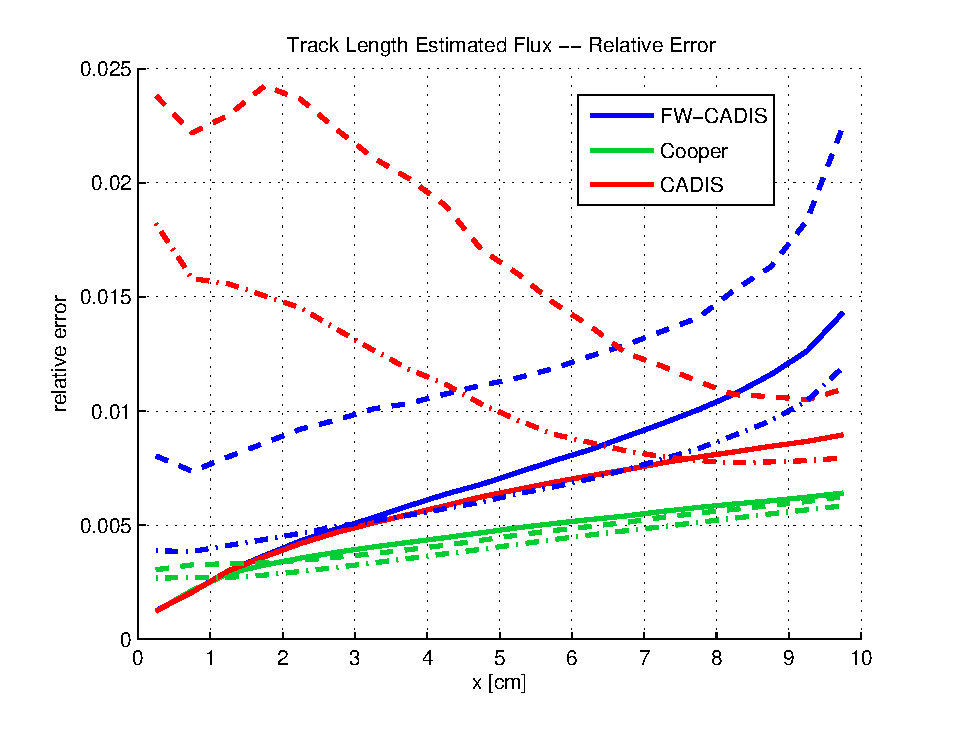
\includegraphics[keepaspectratio, width = 4.0 in]{3gstat}
   \caption{Relative statistical error throughout slab. Solid is group 1, dashed group 2, and dash-dot group 3.}
   \label{fig:3gstat}
\end{figure}

\begin{figure}[!] 
   \centering
   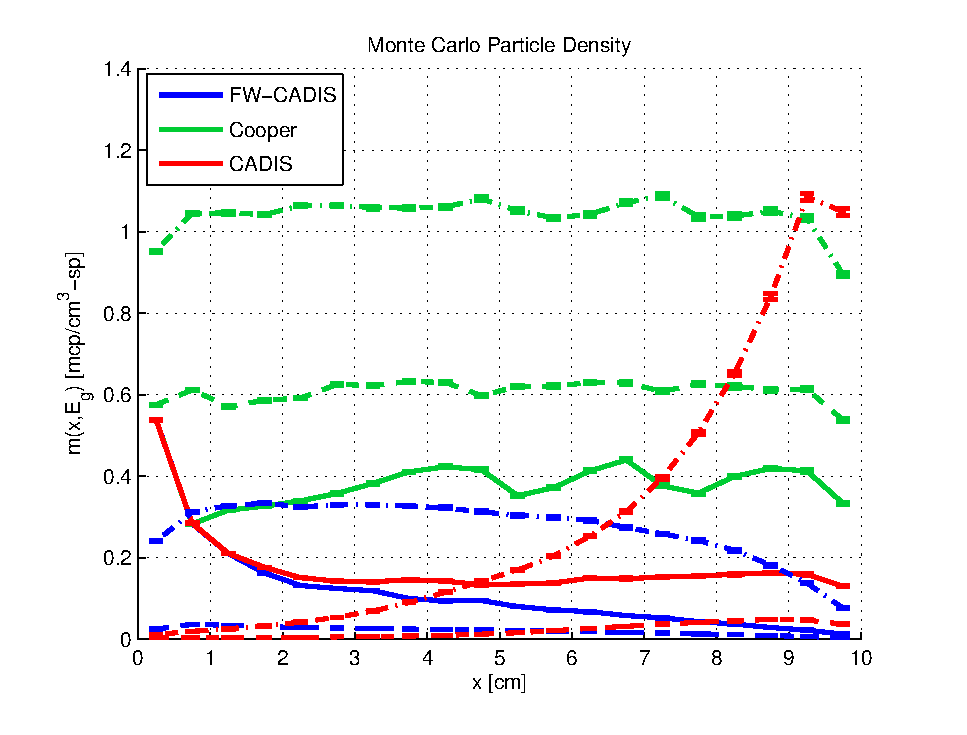
\includegraphics[keepaspectratio, width = 4.0 in]{3gmcps}
   \caption{Monte Carlo particle density throughout slab.  Solid is group 1, dashed group 2, and dash-dot group 3.}
   \label{fig:3gmcps}
\end{figure}

\subsection{Effect of Adjoint Resolution}

A study was performed after the others to see what impact the selection of fine meshing and $S_N$ order has on the variance reduction.  Only the one-group source-detector problem was investigated.  Fine mesh counts of 1, 2, 5, 10, and 20 per coarse mesh were studied for each of $S_N$ orders 2, 4, 8, 16, and 32.  Table \ref{tbl:snmeshstudy} provides the FOM for the far detector using the standard CADIS method.  10$^5$ particles were used in each simulation.

For all fine mesh counts, $S_2$ gives substantially worse results than higher orders.  For higher orders, few fine meshes (\ie large $\Delta x$) give rise to negative angular fluxes, denoted by $*$; for $S_{32}$, a single fine mesh actually gives rise to a negative adjoint scalar flux, denoted by $\varnothing$.  The fluxes appear largely to reduce the effectiveness of the variance reduction, as is expected.  However, the best FOM comes from $S_8$ with just a single mesh.  As implemented, there is a significant trade of between a high resolution and the efficacy of the weight windows.  More fine meshes leads to a slight increase in search time for the weight checking, though this is relatively insignificant in one dimension and even for the more general case of a Cartesian grid.  

\begin{table}[th]
 \caption{Far detector figure-of-merit for several fine meshes and $S_N$ order}
 \begin{center} 
 {\small
 \begin{tabular*}{0.70\textwidth}{@{\extracolsep{\fill}} cccccc } 
  \toprule 
   {\sc $S_N$ / mesh}  &  1  &  2  &  5  &  10  &  20  \\
  \midrule 
   2  & 8.00 & 8.62 & 8.09 & 7.89 & 7.54 \\
   4  & 12.79 & 12.34 & 11.00 & 10.82 & 10.34 \\
   8  & 12.80$^{*}$ & 12.10 & 11.38 & 10.72 & 10.40 \\
   16 & 8.00$^{*}$ & 12.65 & 11.62 & 10.53 & 10.81 \\ 
   32 & 2.23$^{\varnothing}$ & 12.37$^{*}$ & 10.86 & 10.72 & 10.43 \\
  \bottomrule 
 \end{tabular*} 
 }
 \end{center} 
 \label{tbl:snmeshstudy}  
\end{table}



\section{Conclusion}
\label{sec:conc}

This paper has reviewed, implemented, and assessed several automated variance reduction schemes for shielding problems.  While the problems studied are extremely simple, they helped demonstrate the value in using an approximate adjoint or forward flux in biasing particle sources and transport.  

Overall, geometry splitting, CADIS, and pseudo-Cooper performed very well in achieving reasonable statistics in deep problem regions.  More difficult problems in a multidimensional space would likely be required to see more significant differences between the methods.   FW-CADIS and pseudo-Cooper were also compared for a global reduction in variance.  For both global problems considered, pseudo-Cooper far outperformed FW-CADIS.   However, as noted above, the efficacy of pseudo-Cooper may degrade for more complicated problems, where FW-CADIS might become more effective.

One key approximation used in all the methods was to integrate away the angular dependence of the weight windows and importances.  This is done largely to eliminate the very large amount of information associated with angle.  Previous work at LANL led to the AVATAR method which assumes a symmetric angular flux about the current vector, which drastically reduces the information needed \cite{vanriper1997ava}.  Very recent efforts at ORNL have begun included the AVATAR method with the CADIS method for beam port problems, where spatial weight windows are largely ineffective \cite{peplow2010hmc}.  

An interesting project would be to explore other ways of keeping angular information while using less than a full angular flux for weight windows.  One way may be to go beyond the essentially $P_1$-like nature of the AVATAR method and to use higher order moments.  Of course, any useful angular study would probably require a move to two- or even three-dimensional problems.  

{\small
\bibliographystyle{unsrt}
\bibliography{biblio}
}

\newpage

\section*{Appendix A - {\sf sampleinput.m} }
\label{app:input}
{\small
\begin{verbatim}
% SAMPLE INPUT FOR 1-D SLAB TRANSPORT w/ AUTOMATED VARIANCE REDUCTION
%  "sample_input.m"
%  The problem is a uniform slab with either 1 or 3 groups, by user choice.
%  Default setting is standard CADIS with an adjoint source in the farthest
%  0.5 cm of a 10 cm slab.
%
%  J. Roberts, 5/6/2010
clear

% INPUT PARAMETER DEFINITIONS
%   The following provides descriptions of all possible user specified
%   variables for the code.  The sample problem specifications are defined
%   following the subsection of descriptions.
%
%   Problem Specification
%      xcm      = coarse mesh boundaries defining "cells"
%      numg     = number of energy groups
%      numm     = number of materials in cross-section array
%      xsec     = cross-section data for all materials
%                 has the format:
%                       mat 1  --> (T,g1) (A,g1) (S,g1->1) (S,g1->2) ...
%                                  (T,g2) (A,g2) (S,g2->1) (S,g2->2) ...
%                                  ...
%                       mat 2  --> ...
%                 (Isotropic scattering in the lab only!!!)
%      mt       = material assignment for each slab cell
%      src      = group wise source strength for each cell (note, this
%                 is renormalized in the code so that the integrated source
%                 distribution is unity)
%      det      = detector specification; this does two things: 1) it
%                 specifies which locations should get FOM's and 2) it
%                 defines the location (and allows energy-dependence)
%                 of the adjoint source if needed for VR. (The adjoint 
%                 source is the cross-section of the detector if all ones 
%                 are used in a specific region; otherwise, a differenct
%                 energy dependence is obtained (i.e. if only thermal
%                 reactions are of interest).
%      N        = number of histories

    xcm     = [0 1 2 3 4 5 6 7 8 9 10 11 12 13 14 15 16 17 18 19 20]/2;
    numg    = 3;
    numm    = 1;
    mt      = [1  1  1  1  1  1  1  1  1  1  1  1  1  1  1  1  1  1  1  1];
    
    if(numg==3)
    xsec    =  [   1.0  0.3  0.3  0.2  0.2
                   1.5  0.9  0.0  0.4  0.2
                   2.0  0.5  0.0  0.0  1.5 
%                  
                   1.0  0.3  0.3  0.2  0.0
                   5.5  5.9  0.0  0.4  0.2
                   2.0  0.5  0.0  0.0  1.5 ];
    
    src     = [1  0  0  0  0  0  0  0  0  0  0  0  0  0  0  0  0  0  0  0
               0  0  0  0  0  0  0  0  0  0  0  0  0  0  0  0  0  0  0  0  
               0  0  0  0  0  0  0  0  0  0  0  0  0  0  0  0  0  0  0  0];    
                 
    det     = [0  0  0  0  0  0  0  0  0  0  0  0  0  0  0  0  0  0  0  0
               0  0  0  0  0  0  0  0  0  0  0  0  0  0  0  0  0  0  0  0
               0  0  0  0  0  0  0  0  0  0  0  0  0  0  0  0  0  0  0  1];
    else       
    xsec    = [ 1.5      0.5      1.0 ];
               
    src     = [1  0  0  0  0  0  0  0  0  0  0  0  0  0  0  0  0  0  0  0];    
                 
    det     = [0  0  0  0  0  0  0  0  0  0  0  0  0  0  0  0  0  0  0  1];
    end
    
    N       = 1e3;

%   Variance Reduction Options
%      impcapt  = implicit capture [ 0=off, 1=on ]
%      srcbias  = source biasing [ 0=off, 1=on] (note, this requires that
%                 the user modify the appropriate portion of the source
%                 routine; instructions can be found there)
%      geosplt  = cell-based geometry splitting [ 0=off, 1=on ] (note, this
%                 uses the Sn-computed adjoint information)
%      stcadis  = weight windows and source biasing [ 0=off, 1=on ] (note,
%                 this uses the (standard) CADIS approach of Wagner, et al. 
%                 and relies on the adjoint information.  Weight windows 
%                 are specified on a grid independent of the actual 
%                 geometry. 
%      fwcadis  = weight windows and source biasing for global variance
%                 reduction [ 0=off, 1=on ] (note, this uses the
%                 forward-weighted CADIS approach.  Basically, the adjoint
%                 is weighted by a forward flux, and the end result can be
%                 better global statistics (i.e. for multiple or global
%                 tallies) then CADIS alone (which focuses more or less on
%                 a source-detector problem)
%      coopers  = weight windows and source biasing via a method similar
%                 to Cooper's method.  Essentially, the inverse foward flux
%                 is used in place of the adjoing.
%      wcut     = weight cutoff for implicit capture
%      wavg     = average weight for implicit capture (after roulette)
%      mcparts  = along with regular tallies, tally the UNWEIGHTED
%                 particles to estimate the population of monte carlo
%                 particles
%      CAUTION: Using more than one VR option might be bad bad news.

    impcapt = 0;
    srcbias = 0;
    geosplt = 0;
    stcadis = 1;
    fwcadis = 0;
    coopers = 0; 
    wcut    = 0;
    wavg    = 0.5;
    mcparts = 1;

%  Discrete Ordinates Options (in addition to above)
%     xfm    = fine mesh interval for coarse divisions
%     ord    = number of ordinates (2,4,8, or 12)
%     maxit  = maximum iterations
%     maxerr = maximum relative pointwise error in phi

    xfm     = [ 1 1 1 1 1 1 1 1 1 1 1 1 1 1 1 1 1 1 1 1]*10;
    ord     = 32;
    maxit   = 1000;
    maxerr  = 1e-7;    
     
% DO NOT MODIFY BELOW
input   =   struct( 'xcm',      xcm, ...
                    'numslabs', length(xcm)-1, ...
                    'numg',     numg, ...
                    'numm',     numm, ...
                    'xsec',     xsec, ...
                    'mt',       mt, ...
                    'src',      src, ...
                    'det',      det, ...
                    'N',        N, ...
                    'impcapt',  impcapt, ...
                    'srcbias',  srcbias, ...
                    'geosplt',  geosplt, ...
                    'stcadis',  stcadis, ...
                    'fwcadis',  fwcadis, ...
                    'coopers',  coopers, ...
                    'wcut',     wcut, ...
                    'wavg',     wavg, ...
                    'mcparts',  mcparts, ...
                    'xfm',      xfm, ...
                    'ord',      ord, ...
                    'maxit',    maxit, ...
                    'maxerr',   maxerr);
% call driver                
[out,snout] = mcdriver(input);

\end{verbatim}
}

\newpage
\section*{Appendix B - Code Listing}
\label{app:code}

\subsection*{{\sf mcdriver.m} }

{\small

\begin{verbatim}
function [finout,snout] = mcdriver(in)
% function mcdriver(in)
%   This function takes as input the struct "in" containing all relevant
%   input parameters from the input file.  Driver then calls the
%   appropriate ''subroutines'' en route to the solution.

    disp('------------------------------------------------------')
    disp('--------- MULTI-GROUP SLAB MONTE CARLO WITH  ---------')
    disp('----- AUTOMATED ADJOINT-BASED VARIANCE REDUCTION -----')
    disp('------ Term Project for 22.106 by J. A. Roberts ------')
    disp('------------------------------------------------------')

% forward discrete ordinates -- used for comparison and possible vr
snout = sndriver(in);
disp('...finished forward SN')

% unbiased source distribution -- takes geometry and makes source densities
srcout = srcdriver(in);
disp('...finished source driver')

% variance reduction -- computes any required vr parameters
[vrout,snout] = vrparm(in,snout,srcout);
disp('...finished vr parameter production')

% play the game -- perform the monte carlo simulation
out = mcslab1d(in,srcout,vrout);
disp('...finished the game and now printing...')

% plots and such
finout = out1d(in,out,snout,srcout,vrout);


end
\end{verbatim}
}

\subsection*{{\sf sndriver.m} }

{\small
\begin{verbatim}
function snout = sndriver(in)
% function snout = sndriver(in)
%    This function takes as input the struct "in" which is defined in the
%    sample input.  The function calls the local function sn_one_d.
%    J. Roberts, 4/13/2010

% compute the forward quantities
tic

[snout.phiF,snout.psiF,snout.phiFplot,snout.phiFavg,snout.xww,snout.x] = ...
    sn_one_d(in,0);

snout.snt = toc;

end

\end{verbatim}
}


\subsection*{ {\sf sn\_one\_d.d } }

{\small
\begin{verbatim}

function [phi,psi,phiPLOT,phiAVG,xe,xa] = sn_one_d(in,adj,qad)

%!!!!!!!!!!!!!!!!!!!!!!!!!!!!!!!!!!!!!!!!!!!!!!!!!!!!!!!!!!!!!!!!!!!!!!!!!!
% This function solves the 1-D multigroup SN equations given input.  It's !
% output is the forward (or adjoint) angular fluxes at the cell edges and !
% the cell-centered scalar flux.  It has been verified against PARTISN for!
% some simple problems.
% ** last modified by J. Roberts, 4/11/2010
%!!!!!!!!!!!!!!!!!!!!!!!!!!!!!!!!!!!!!!!!!!!!!!!!!!!!!!!!!!!!!!!!!!!!!!!!!!

% 1) struct "in" contains (among other things)
%     numg   = number of energy groups
%     numm   = number of materials
%     xcm    = coarse divisions
%     xfm    = fine mesh interval for coarse divisions
%     mt     = material assignment for each coarse division
%     xsec   = cross-sections in the form
%              (mat1/g1) sigTOT   sigA  sigSg1->g1  sigSg1->g2 ...
%                 ...g2) sigTOT   sigA  sigSg2->g1  ....
%              (mat2/g1) ...
%     src    = volumetric (isotropic) source by coarse mesh and energy
%              (for adj, src is the cross-section for the source region)
%     det    = spatial location of detector
%     ord    = number of ordinates (2,4,8, or 12)
%     maxit  = maximum iterations
%     maxerr = maximum relative pointwise error in phi
% 2)  adj    = 0-->forward, 1-->adjoint
% 3)  qad    = if present, it is a fine mesh adjoint source
% working variables
%     dx     = fine mesh divisions
%     mtt    = material assignment for fine mesh cells
%     n      = number of fine mesh cells

numg = in.numg;
ord  = in.ord;
Q = zeros(  sum(in.xfm), ord, numg );

bound       =   [ord/2+1 ord; 1 ord/2];
gbound      =   [ 1  numg];
git         =   1;
S           =   in.src;
if adj == 1
    git         = -1;
    gbound      = [numg 1];
    bound       = flipud(bound);
    % define S to be the group-wise TOTAL cross section in the detector
    S = in.det;
%     for i = 1:length(in.xfm) % number of course meshes
%         for g = 1:numg
%         	S(g,i) = in.det(g,i)*in.xsec((in.mt(i)-1)*numg+g, 1);
%         end
%     end
end

% -------------------------------------------------------------------------
% -------------------------------------- Discretizations
[mu,w] = S_1D(in.ord);
j = 0;
for i = 1:length(in.xfm)
    dx( (j+1):(j+in.xfm(i))   )  = (in.xcm(i+1)-in.xcm(i))/in.xfm(i);
    if nargin == 2
        for g=gbound(1):git:gbound(2)
            Q( (j+1):(j+in.xfm(i)), :, g)  = S(g,i);
        end
    else
        for g=gbound(1):git:gbound(2)
            for k = 1:ord
                Q( (j+1):(j+in.xfm(i)),k,g)  = qad((j+1):(j+in.xfm(i)),g);
            end
        end
    end
    mtt( (j+1):(j+in.xfm(i))   )  = in.mt(i);  % assign mat to each f mesh
    j = sum(in.xfm(1:i));
end
n = sum(in.xfm);

% -------------------------------------------------------------------------
% -------------------------------------- Matrix Pre-allocation
psi         =   zeros(n+1,ord,numg);        % Angular Flux
cur         =   zeros(n,numg);              % Current
phi_o       =   zeros(n,numg);              % Scalar Flux Old
phi         =   zeros(n,numg);              % Scalar Flux New
con1        =   zeros(n,ord,numg);          % Transport Coef.
con2        =   zeros(n,ord,numg);          % Transport Coef.
con3        =   zeros(n,ord,numg);          % Transport Coef.
q           =   zeros(n,ord,numg);          % Scattered Source

% -------------------------------------------------------------------------
% -------------------------------------- Transport Coefficients
for g = gbound(1):git:gbound(2)
    for k = 1:n
        m = mtt(k);
        con1(k,:,g) = in.xsec((m-1)*numg+g,1)*dx(k)./(2.0*mu(:));
        con2(k,:,g) = (1.0-sign(mu(:)').*con1(k,:,g))./...
            (1.0+sign(mu(:)').*con1(k,:,g));
        con3(k,:,g) = sign(mu(:)').*dx(k)./(mu(:)'.*...
            (1.0+sign(mu(:)').*con1(k,:,g)));
    end
end

q = Q;

% ----------------- Solution Algorithm ------------------------------------

for g = gbound(1):git:gbound(2)
    
    % ----------------- Convergence Parameters ----------------------------
    err  = 10;
    iter = 0;
    
    while err > in.maxerr && iter < in.maxit
        % -------------------------------------- Mu > 0
        for k = 1:1:n
            for j = bound(1,1):bound(1,2)
                psi(k+1,j,g) = psi(k,j,g)*con2(k,j,g)+q(k,j,g)*con3(k,j,g);
            end
        end
        % -------------------------------------- Mu < 0
        for k = n:-1:1
            for j = bound(2,1):bound(2,2)
                psi(k,j,g) = psi(k+1,j,g)*con2(k,j,g)+q(k,j,g)*con3(k,j,g);
            end
        end
        
        % ---- Scalar Flux
        for k = 1:n
            phi(k,g) = sum(w'.*0.25.*(psi(k,:,g)+psi(k+1,:,g)));
        end
        % ---- Updated Source Term
        for z   =   g:git:gbound(2) % only down scattering
            for kk = 1:n
                q(kk,:,z) = Q(kk,:,z); % reset
            end
            if adj == 0
                for k = 1:n
                    m = mtt(k);
                    for gg = gbound(1):git:gbound(2) % group gg to group z
                        q(k,:,z) = q(k,:,z) + ...
                            in.xsec((m-1)*numg+gg,2+z)*phi(k,gg);
                    end
                end
            else
                for k = 1:n
                    m = mtt(k);
                    for gg = gbound(1):git:gbound(2) % group gg to group z
                        q(k,:,z) = q(k,:,z) + ...
                            in.xsec((m-1)*numg+z,2+gg)*phi(k,gg);
                    end
                end
            end
        end
        % ---- Scalar Flux Error Between Iterations
        err = max(max(abs(phi-phi_o)./phi));
        % ---- Reset Scalar Flux
        phi_o = phi;
        % ---- Iteration Counter
        iter = iter + 1;
    end
    
end

% stuff for future plotting: phiPLOT is a step-wise phi, and phiAVG is the
% average value for a coarse mesh region (for comparison to MC values)


xa(1)=dx(1)/2+in.xcm(1);
for i = 2:length(dx)
    xa(i) = xa(i-1) + 0.5*(dx(i-1)+dx(i));
end
xe(1)=in.xcm(1);
for i = 2:length(dx)+1
    xe(i) = xe(i-1) + dx(i-1);
end

    
for g = 1:in.numg
    j=0;
    for i = 1:length(in.xfm)
        phiPLOT( (j+1):(j+in.xfm(i)), g)  = ...
            mean( phi( (j+1):(j+in.xfm(i)) , g) ) ;
        phiAVG(i,g)   = mean( phi( (j+1):(j+in.xfm(i)) , g) );
        j = sum(in.xfm(1:i));
    end
end

if sum(sum(phi<0)) > 0
    if (adj==1)
        disp('*** warning: negative adjoint')
    else
        disp('*** warning: negative forward')
    end
    disp('     make smaller mesh size or turn on')
    disp('     negative flux fixup')
end
if sum(sum(sum((psi<0)))) > 0
    if (adj==1)
        disp('*** warning: negative angular adjoint')
    else
        disp('*** warning: negative angular forward')
    end
    disp('     make smaller mesh size or turn on')
    disp('     negative flux fixup')
end

end

\end{verbatim}
}

\subsection*{{\sf srcriver.m} }

{\small
\begin{verbatim}

function srcout = srcdriver(in)
% function srcout = srcdriver(in)
%   This function produces the unbiased source density
%   for use in the simulation.  Its basic output is the
%   cell/energy discrete pdf.

% source biasing
    %  Here, we need to look at the volumetric source distribution
    %  as well as the fine mesh adjoint
    if in.numg>1
        srcloc = find(sum(in.src)>0); % picks out cell numbers w/ src
    else
        srcloc = find(in.src>0);
    end
    denom = 0;
    
    for i = 1:length(srcloc)
        V(i) = in.xcm( srcloc(i)+1)-in.xcm( srcloc(i) );
        sx(i,1)=in.xcm( srcloc(i) ); % lower bound
        sx(i,2)=in.xcm( srcloc(i)+1); % upper bound
        denom = denom + V(i)*sum( in.src(:,srcloc(i)));  
    end
    for i = 1:length(srcloc)
        P(1:in.numg,i)=V(i)*in.src(1:in.numg, srcloc(i))/denom;    
    end
    % P gives a cell/energy-dependent source density
    %   To use this in an unbiased source, so the following:
    %       Px = sum(P) --> cell dependent probability
    %       for i=1,numsrccell, if rand < sum(Px(1:i)), found cell
    %        x = rand*(dx(i,2)-dx(i,1))+dx(i,1)
    %       for j=1,numg, if rand < sum(Px(i,j)), found group
    %        g = j;
    if in.numg > 1
        Px=sum(P);
    else
        Px = P;
    end
    numsrc=length(srcloc);
    
    srcout   =   struct( 'srcloc', srcloc, ...
                         'numsrc', numsrc, ...
                         'sx',     sx, ...
                         'P',      P, ...
                         'Px',     Px, ...
                         'nrmfct', denom);
end

\end{verbatim}
}

\subsection*{{\sf vrparm.m} }

{\small
\begin{verbatim}
function [vrout,snout] = vrparm(in,snout,srcout)
% function vrout = vrparm(in,snout)
%   This function generates any needed variance reduction parameters
%   required for the adjoint-based approaches (i.e. geometry splitting, or
%   either of the CADIS approaches.  Only one can be used!
tic

vrout.imp = 0;
% For reference, review the basic ideas of each variance reduction method
% option that uses the adjoint.
%
% Geometry Splitting 
%     Reference:  F.B. Brown, "Fundamentals of Monte Carlo Particle
%                 Transport", LA-UR-05-4983
%     In geometry splitting, an importance is assigned to each cell.  When
%     a neutron leaves cell a with importance ia, and goes to cell b with
%     importance ib, either ia<ib or ia>ib (or possibly, though unlikely,
%     ia=ib).  Then we let
%                  r = ib/ia   
%                  if r > 1
%                    n = floor(r)
%                    if n > 1
%                       split into n particles of w = w/n
%                       and each particle has the same (x,mu,g,...)
%                    end
%                  else % r < 1
%                    if rand < r
%                      w = w/r
%                    else
%                      kill particle
%                    end
%                  end
%     Note, it may or may not be wise to implement a weight cutoff with
%     splitting.
%
%  Parameters:
%     imp   = cell energy-dependent importances (just average adjoint
%             scalar flux over cell)
if in.geosplt==1

    % compute the adjoint
    [snout.phiA,snout.psiA,snout.phiAplot,snout.phiAavg,snout.xww] = ...
            sn_one_d(in,1);

    % the importance is just the average adjoint flux i.e. cell importance
    vrout.imp = snout.phiAavg;

% CADIS (Consistent Adjoint-Driven Importance Sampling
%     Reference: J.C. Wagner and A. Haghighat, "Automated Variance
%                Reduction of Monte Carlo Shielding Calculations Using the
%                Discrete Ordinates Adjoint Function", Nuclear Science and
%                Engineering, 128, 186-208 (1998)
%     The CADIS method does two things: it biases the transport of
%     particles via weight windows, and it biases the source so that
%     particles are born with weights withing their local weight window,
%     i.e. with consistent weights.  This consistency makes the method much
%     more efficient.  Note, while the underlying adjoint can theoretically
%     be a global one, CADIS works best for simple source-detector
%     problems.
%
%     Source Biasing
%          The source energy and position are sample from a biased source
%          distribution defined as:
%               q*(r,E)  =  [ phiA(r,E)*q(r,E) ] / < phiA(r,E)*q(r,E) >
%                        =  [ phiA(r,E)*q(r,E) ] / R
%          where "< >" means integration over all space and energies.  The
%          denominator is the total detector response.  Because the source
%          particles are biased, their weights are defined to be:
%                W(r,E)  =  R/phiA(r,E)
%          Note, "phiA" is the adjoint scalar flux.
%     Transport Biasing
%          First, recall the idea of weight windows.  For a particular cell
%          i, upper and low weight windows (wU and wL) are defined.  If a
%          particle of weight w enters cell i, we have three possibilities:
%          1) w < wL, 2) w>wU, or 3) wL<w<wU.  In the third case, nothing
%          happens, but case 1) leads to roulette and 2) leads to
%          splitting.  Here's the algorithm:
%               if w > wU
%                 n = min(mxspln, 1+wgt/wU) <- mxspln is max split ratio
%                 w = w/n
%                 bank n-1 copies, and follow the current particle
%               elseif w < wL
%                 P = max(1/mxspln, w/wavg) <= wavg is avg w 
%                 if rand < P
%                   w = w/P
%                 else
%                   kill particle
%                 end
%               end
%          Now to choose the wU and wL values we use CADIS, and so we have:
%               wL(r,E) =  [R/phiA(r,E)] * [2/(cU + 1)] 
%          where cU defines the width such that cU=wU/wL.  The default cU
%          in MCNP is 5.  We use that here, too.
elseif (in.stcadis+in.fwcadis+in.coopers) > 0
    
    % SOURCE BIASING
    
    %  step 1.  reconstruct unbiased source density mapped onto fine grid
    %     Recall that P is the cell/energy discrete source density
    %     in the form [ p(c1,g1)  p(c2,g1) ...
    %                   p(c1,g2) ...
    %     with corresponding cell bounds given by sx(ci,1) and sx(ci,2).
    %     What we need is a new discrete density corresponding to the same
    %     source mapped onto the fine grid defined by in.xfm.  Within a
    %     (coarse) cell, the source is uniformly distributed, and so should
    %     it be in a fine cell; hence, the probabilities for the fine cells
    %     will be just the original (coarse) probability divided by the
    %     number of fine cells, and the total number of columns of the new
    %     (still unbiased) source vector will be the total number of fine
    %     meshes in all source cells.  Hence,
    Pf  = zeros(in.numg, sum(in.xfm(srcout.srcloc)) );
    sxf = zeros(sum(in.xfm(srcout.srcloc)), 2);
    j = 0;
    for i = 1:length(srcout.srcloc)
        ii = srcout.srcloc(i);
        for g = 1:in.numg
            Pf( g, (j+1):(j+in.xfm(ii)) )  = ...
                srcout.P(g,i)/in.xfm(ii);
        end
        dx = ( srcout.sx(i,2)-srcout.sx(i,1) ) / in.xfm(ii);
        for k = 1:in.xfm
            sxf(j+k,1) = (k-1)*dx + srcout.sx(i,1);
            sxf(j+k,2) = dx+sxf(j+k,1);
        end
        j = j+in.xfm(ii);
    end
    
    %  step 2.  bias the resulting density and produce weights

    % compute the adjoint
    if in.stcadis == 1
        [snout.phiA,snout.psiA,snout.phiAplot,snout.phiAavg] =...
            sn_one_d(in,1);
    elseif in.fwcadis == 1
        [snout vrout] = fwcadis(in,snout,srcout,vrout);
    elseif in.coopers == 1
        %[snout.phiA,snout.psiA,snout.phiAplot,snout.phiAavg] =...
        %    sn_one_d(in,1);        
        snout.phiA = 1./snout.phiF;
    end
    
    pfbias = zeros(size(Pf)); % temporary
    weight = pfbias;
    for i = 1:srcout.numsrc
        % pick out the adjoint corresponding to this source location
        if srcout.srcloc(i) > 1
            step = sum( in.xfm(1:srcout.srcloc(i)-1) );
        else
            step = 0; step2 = 0;
        end
        pfbias(:,step2+1:step2+in.xfm(srcout.srcloc(i))) = ...
            ( snout.phiA(step+1:step+in.xfm(i),:).*...
              Pf(:,step2+1:step2+in.xfm(srcout.srcloc(i)))' )';
        weight(:,step2+1:step2+in.xfm(srcout.srcloc(i))) = ...
                1 ./ snout.phiA(step+1:step+in.xfm(i),:)';
        step2 = step2 + in.xfm(srcout.srcloc(i));
    end
    R      = sum(sum(pfbias)); % R is just the sum of all the q*phi's
    Pf     = pfbias / R;       % and we renormalize our source density
    Pfx    = sum(Pf);
    weight = weight * R;       % and our weights.

    vrout.Pf     = Pf;
    if (in.numg>1)
        vrout.Pxf = sum(Pf);
    else
        vrout.Pxf = Pf;
    end
    vrout.sxf    = sxf;
    vrout.weight = weight;
    vrout.numsrc = length(vrout.Pxf);
    
    % TRANSPORT BIASING (...remarkably more straightforward!)
    %   wL(r,E) =  [R/phiA(r,E)] * [2/(cU + 1)]
    vrout.xww(:,1) = snout.xww(1:end-1)';
    vrout.xww(:,2) = snout.xww(2:end)';
    vrout.cU = 5.0; % default ratio of upper and lower bounds
    vrout.wL = (2*R/(vrout.cU+1))./snout.phiA;
    
end

vrout.t = toc; % total vr parameter generation time
end

function [snout vrout] = fwcadis(in,snout,srcout,vrout)
% FW-CADIS (Forward-Weighted CADIS)
%     Reference: J.C. Wagner et al. "Forward-Weighted Cadis Method for
%                Variance Reduction of Monte Carlo Calculations of 
%                Distributions and Multiple Localized Quantities",
%                International Conference on Mathematics, Computational
%                Methods, and Reactor Physics (M&C 2009)
%          The basic idea of CADIS remains, but a minor modification is
%          made.  Instead of the original adjoint source, a forward
%          flux-weighted adjoint source is used.  For example, if our
%          desired "response" is uniform statistical error throughout the
%          problem, then (see the reference) it can be shown that we want
%                             Qadj(r,E) = 1 / phiF(r,E)
%          Of course, phiF is exactly what we aim to calculate!  But here, 
%          of course, we use a crude SN approximation for it.
%
%          Because the only difference between CADIS and FW-CADIS is the 
%          adjoint source used to generate the adjoint fluxes, FW-CADIS is
%          implemented here essentially as an optional subroutine called
%          from within the CADIS routine above.
    
    % first build the coarse adjoint distribution
    if in.numg>1
        srcloc = find(sum(in.det)>0); % picks out cell numbers w/ src
    else
        srcloc = find(in.det>0);
    end
    denom = 0;
    for i = 1:length(srcloc)
        V(i) = in.xcm( srcloc(i)+1)-in.xcm( srcloc(i) );
        sx(i,1)=in.xcm( srcloc(i) );  % lower bound
        sx(i,2)=in.xcm( srcloc(i)+1); % upper bound
        denom = denom + V(i)*sum( in.det(:,srcloc(i)));  
    end
    for i = 1:length(srcloc)
        P(1:in.numg,i)=V(i)*in.det(1:in.numg, srcloc(i))/denom;    
    end
    if in.numg > 1
        Px=sum(P);
    else
        Px = P;
    end
    numsrc=length(srcloc);
    % then build the fine adjoint distribution
    Pf  = zeros(in.numg, sum(in.xfm(srcloc)) );
    sxf = zeros(sum(in.xfm(srcloc)), 2);
    j = 0;
    for i = 1:length(srcloc)
        ii = srcloc(i);
        for g = 1:in.numg
            Pf( g, (j+1):(j+in.xfm(ii)) ) = P(g,i)/in.xfm(ii);
        end
        dx = ( sx(i,2)-sx(i,1) ) / in.xfm(ii);
        for k = 1:in.xfm
            sxf(j+k,1) = (k-1)*dx + sx(i,1);
            sxf(j+k,2) = dx + sxf(j+k,1);
        end
        j = j+in.xfm(ii);
    end
    % now weight the adjoint distribution with the forward flux
    qad = zeros(size(snout.phiF));
    step = 0; step2 = 0;
    for i = 1:numsrc
        % pick out the adjoint corresponding to this source location
        if srcloc(i) > 1
            step = sum( in.xfm(1:srcloc(i)-1) );
        else
            step = 0; step2 = 0;
        end
        qad(step+1:step+in.xfm(i),:) = ...
          ( Pf(:,step2+1:step2+in.xfm(srcloc(i)))' ./ ...
            snout.phiF(step+1:step+in.xfm(i),:) );
        step2 = step2 + in.xfm(srcloc(i));
    end
    % now calculate the adjoint using the weighted adjoint source
    [snout.phiA,snout.psiA,snout.phiAplot,snout.phiAavg,snout.xww] = ...
            sn_one_d(in,1,qad);

end


\end{verbatim}
}

\subsection*{{\sf mcslab1d.m} }

{\small
\begin{verbatim}
function output = mcslab1d(in,srcout,vrout)
% function output = mcslab1d(in,vrout)
%   This function performs multi-group Monte Carlo particle transport in a
%   1-D Cartesian slab.
%
% J. Roberts 4/13/2010

	tic
	
	% initialize flux estimators
	trakest = zeros(2, in.numslabs, in.numg);
	collest = zeros(2, in.numslabs, in.numg);
    % monte carlo particle population estimator
    if in.mcparts == 1
        mcpest = zeros(2, in.numslabs, in.numg);
    end
    
    ww = in.stcadis+in.fwcadis+in.coopers; % >0 to check ww's

	minw = 1;
    
    %%%%%%%%%%%%%%%%% BEGIN HISTORIES %%%%%%%%%%%%%%%%%%%%%%%%%%%%%%%%%%%%%
    for n = 1:in.N % histories

        % Call source() to get my starting location and direction.  Because
        % source biasing may yield several particles, I've got to have a
        % bank of neutrons associated with history "n".  This bank will be
        % useful for geometry splitting and weight windows, too.
        [x,mu,g,ps,wt] = source(in,srcout,vrout);
        bank(1:ps,:) = [ x mu g wt ];
        
        % reset (or initialize) temporary tallies
        tmptrak = zeros(1,in.numslabs,in.numg);
        tmpcoll = zeros(1,in.numslabs,in.numg);
        tmpmcp  = zeros(1,in.numslabs,in.numg);
        
        while length(bank(:,1)) >= 1 % go through entire bank
           % if length(bank(:,1))>10000
           %     disp('whoa!')
           %     return
           % end
            x  = bank(1,1);  % my start location
            mu = bank(1,2);  % my start direction
            g  = bank(1,3);  % my energy group
            w  = bank(1,4);  % my weight
            alive = 1;       % i am alive
            coll = 0;        % i am not exiting a collision
            mycell = getmycell(x,in);  % get my cell
            
            while alive == 1;
                
                % post collision stuff
                if coll == 1
                    % i need a new direction in life
                    mu = 2*rand-1; % we're isotropic
                    % i also need a new energy 
                    % sct gives me the vector of g->g' sigs where I am g
                    sct = in.xsec( in.numg*(in.mt(mycell)-1)+g, 3:end);
                    sct = sct/sum(sct); % normalize for prob.
                    ksi = rand;
                    for i = 1:length(sct)
                        if ksi < sum(sct(1:i))
                            g = i;
                            break
                        end
                   end           
                end
                
                % check weight window if needed
                if ww>0
                   [w,bank,alive] = wwcheck(x,mu,g,w,bank,vrout);
                   if alive == 0
                       break
                   end
                end   
                
                % determine my neighbor and how far to her
                [neighbor,d2neighbor] = getmyneighbor(mycell,x,mu,in);
                
                % sample how many mfp's I will go
                ksi = rand;
                mfps = -log(ksi);
                
                % determine my total cross-section
                SigT = in.xsec( in.numg*(in.mt(mycell)-1)+g, 1);
                
                % determine how far along x-axis I go
                dist = mfps*mu/SigT;
                
                % determine whether I reach surface
                if ( abs(dist) > d2neighbor) % then I pass to the next cell
                    tmptrak(1,mycell,g)=tmptrak(1,mycell,g)+...
                        w*abs(d2neighbor/mu);
                    if  (neighbor==0)
                        % I leaked out of left
                        alive=0;
                    elseif (neighbor==in.numslabs+1)
                        % I leaked out of right
                        alive=0;
                    else % i simply get to the boundary
                        % and i may or may not be split or rouletted
                        x = x+sign(mu)*d2neighbor;
                        if in.geosplt == 1 && neighbor > 0 ...
                                           && neighbor < in.numslabs+1     
                          [w,bank,alive] = ...
                              splitme(neighbor,mycell,x,mu,g,w,bank,vrout);
                        end
                        mycell = neighbor;
                        coll = 0;
                    end
                else
                    % otherwise, I collide; no matter what collision we
                    % have, tally my incoming weight
                    tmpcoll(1,mycell,g) = tmpcoll(1,mycell,g)+w;
                    tmptrak(1,mycell,g) = tmptrak(1,mycell,g)+w*mfps/SigT;
                    if in.mcparts == 1
                    	tmpmcp(1,mycell,g)  = tmpmcp(1,mycell,g)+1; 
                    end
                    
                    % update my location
                    x = x+dist;
                    if in.impcapt == 1
                        % reduce my weight
                        w = w*(1-in.xsec(in.numg*(in.mt(mycell)-1)+g,2)...
                            /SigT);
                        coll = 1;
                        % check to see if weight is below cutoff
                        if w < in.wcut
                            if rand < w/in.wavg
                                w = in.wavg;
                            else
                                alive = 0;
                                break;
                            end
                        end
                    else
                        if rand < in.xsec(in.numg*(in.mt(mycell)-1)+g,2)...
                                /SigT;
                            % i am absorbed
                            alive = 0;
                        else
                            % i am scattered;
                            coll = 1;
                        end
                    end
                end

            end
            % end while alive
            
            if length(bank(:,1)) > 1 % reduce the bank
                bank = bank(2:end,:);
            else % else, we'll go to the next history
                break
            end
            
        end
        % end while bank
        
        % update tallies
        for i = 1:in.numg
            collest(1,:,i) = collest(1,:,i) + tmpcoll(1,:,i);
            collest(2,:,i) = collest(2,:,i) + tmpcoll(1,:,i).^2;
            trakest(1,:,i) = trakest(1,:,i) + tmptrak(1,:,i);
            trakest(2,:,i) = trakest(2,:,i) + tmptrak(1,:,i).^2;
            if in.mcparts==1
                mcpest(1,:,i) = mcpest(1,:,i) + tmpmcp(1,:,i);
                mcpest(2,:,i) = mcpest(2,:,i) + tmpmcp(1,:,i).^2;
            end
        end

    end
    %%%%%%%%%%%%%%%%% END OF HISTORIES %%%%%%%%%%%%%%%%%%%%%%%%%%%%%%%%%%%%
    
	%disp(['minw=',num2str(minw)])  
	t2 = toc;
	output = struct(  'trakest',    trakest, ...     % track length est
                      'collest',    collest, ...     % collision est
                            't',          t2 ...     % finish time
	);    
    if in.mcparts==1
       output.mcpest = mcpest; 
    end
end
% end function playgame

function [x,mu,g,ps,wt] = source(in,srcout,vrout)
	% In this function, the source distribution is assigned.
 
    % Analog Source
    %   Here, we use the pre-generated source distribution vectors
    %   from srcdriver.  Px is the discrete pdf if a particle is born
    %   (uniformly) within a given slab cell.  Once that cell is
    %   selected, x is sampled uniformly within the cell.  Then
    %   the group is sampled within that cell using 
    %      p(group|cell) = p(group,cell)/p(cell) = p(:,i)/Px(i)
    if (in.srcbias + in.stcadis + in.fwcadis + in.coopers) == 0
        
        g=-1; x=-1;
        ksi1 = rand;
        for i = 1:srcout.numsrc
            if ksi1 < sum(srcout.Px(1:i))
                x = rand*(srcout.sx(i,2)-srcout.sx(i,1))+srcout.sx(i,1);
                break
            end
        end
        ksi2 = rand;
        for j = 1:in.numg
            if ksi2 < sum(srcout.P(1:j,i))/srcout.Px(i)
                g = j;
                break
            end
        end
        if g==-1 || x == -1
            disp('kaka')
        end
        mu = 2*rand-1;
        wt = 1;
        ps = 1;

    elseif ( in.stcadis + in.fwcadis + in.coopers ) > 0
        
        g=-1; x=-1;
        ksi1 = rand;
        for i = 1:vrout.numsrc
            if ksi1 < sum(vrout.Pxf(1:i))
                x = rand*(vrout.sxf(i,2)-vrout.sxf(i,1))+vrout.sxf(i,1);
                break
            end
        end
        if in.numg > 1
            ksi2 = rand;
            for j = 1:in.numg
                if ksi2 < sum(vrout.Pf(1:j,i))/vrout.Pxf(i)
                    g = j;
                    break
                end
            end
        else
            g = 1;
        end
        if g == -1 || x == -1
            disp('source issue!')
        end
        mu = 2*rand-1;
        wt = vrout.weight(g,i);
        ps = 1;
    end
        
    % MANUAL SOURCE BIASING 
    %   feel free to add me
end
% end function source

function [neighbor, d2neighbor] = getmyneighbor(mycell,x,mu,in)
    % mycell is my current cell, and neighbor is the one i'd enter
    if mu > 0
        d2neighbor = (in.xcm(mycell+1)-x);
        neighbor=mycell+1;
    else
        d2neighbor = (x-in.xcm(mycell));
        neighbor=mycell-1;
    end
end
% end function getmyneighbor

function [mycell] = getmycell(x,in)
    for mycell = 1:in.numslabs
        if x < in.xcm(mycell+1)
            break
        end
    end
end
% end function mycell

function [w,bank,alive] = wwcheck(x,mu,g,w,bank,vrout)
    alive = 1;
    % first find my wL
% linear search:  (r
%     for i = 1:length(vrout.xww(:,1))
%         if x < vrout.xww(i,2)
%             wL = vrout.wL(i,g);
%             wU = vrout.cU*wL;
%             break
%         end
%     end
    i = binsearch(x,vrout.xww(:,2),mu); %mu used to correct index at bound
    wL = vrout.wL(i,g); wU = vrout.cU*wL;
    if w > wU
%         r = w/wU; % NEW
%         if rand < r-floor(r)
%             n = ceil(r);
%         else
%             n = floor(r);
%         end
%         w = w/n;
%         if n > 1
%           bank(end+1:end+n-1,:) = ...
%             [ ones(n-1,1)*x ones(n-1,1)*mu ones(n-1,1)*g ones(n-1,1)*w ];
%         end
        n = floor(1+w/wU); % OLD
        if n > 1
            w = w/n;
            % bank n-1 particles
            bank(end+1:end+n-1,:) = ...
             [ ones(n-1,1)*x ones(n-1,1)*mu ones(n-1,1)*g ones(n-1,1)*w ];
        end
    elseif w < wL
        P = 2*w/(wU+wL); % i.e. the average w is in the center
        if rand < P
            w = w/P;
        else
            alive = 0;
        end
    end
end
% end function wwcheck

function index = binsearch(x,F,mu)
    % simple binary search for use in source sampling and wwcheck
    L = 1;  R = length(F);
    while(1)
        M = round( (L+R)/2 );
        if x > F(M)
            L = M+1;
        elseif x < F(M)
            R = M-1;
        else
            index=M+(mu>0);
            break
        end
        if ( L>R)  % end of search; determine which side we end on
            if F(M) > x
                index=M;
            else
                index=M+1;
            end
            break
        end
    end
end
% end function binsearch

function [w,bank,alive] = splitme(neighbor,mycell,x,mu,g,w,bank,vrout)
    alive = 1;
    r = vrout.imp(neighbor,g)/vrout.imp(mycell,g);
    if (r > 1.0) % split
        if rand < r-floor(r)
            n = ceil(r);
        else
            n = floor(r);
        end
        w = w/r;
        if n > 1
          bank(end+1:end+n-1,:) = ...
            [ ones(n-1,1)*x ones(n-1,1)*mu ones(n-1,1)*g ones(n-1,1)*w ];
        end
    else % russian roulette
        if rand < r
            w = w/r;
        else
            alive = 0;
        end
    end
end
% end function splitme



\end{verbatim}
}

\subsection*{{\sf out1d.m} }

{\small
\begin{verbatim}
function finout = out1d(in,out,snout,srcout,vrout)
% function out1d(in,out,snout)
%   This function manipulates the tallies from the simulation into the
%   fluxes or reaction rates required.  It computes figure-of-merits.  It
%   plots the Monte Carlo results and the (forward) discrete ordinates
%   results.

	disp(['  Monte Carlo elapsed time: ', num2str(out.t)])
    disp(['   Forward SN elapsed time: ', num2str(snout.snt)])
    if ( in.geosplt+in.stcadis+in.fwcadis+in.coopers > 0 )
        if in.fwcadis == 1
            vrout.t=vrout.t+snout.snt;
        end
        if in.coopers == 1
            vrout.t=vrout.t+snout.snt;
        end
        disp(['    VR Param. elapsed time: ', num2str(vrout.t)])
    end
    disp(' Variance Reduction: ')
    if in.impcapt == 1, disp(' * implicit capture'), end
    if in.srcbias == 1, disp(' * manual source biasing'), end
    if in.geosplt == 1, disp(' * adjoint-based geometry splitting'), end
    if in.stcadis == 1, disp(' * standard cadis'), end
    if in.fwcadis == 1, disp(' * forward-weighted cadis'), end
    if in.coopers == 1, disp(' * pseudo coopers'), end
    
    [phi1,re1]   = phi_tl(in,out);
    [phi2,re2]   = phi_cd(in,out);

%     if in.mcparts == 1
%         out.collest = out.mcpest;
%         [phiMC,reMC] = phi_cd(in,out);
%     end
    
    if in.mcparts == 1
    	[phiMC,reMC] = phi_mc(in,out);
    end
        
    finout.t=out.t+vrout.t;
    % now print the fluxes all nice
    for g = 1:in.numg
    disp([' group ',num2str(g)])
\end{verbatim}
}
{\footnotesize
\begin{verbatim}
    disp(' reg   |     phi1       RE         FOM    |     phi1       RE         FOM   | ')
    disp('-----------------------------------------------------------------------------')
    for i = 1:in.numslabs
        if in.det(g,i) > 0 % point an arrow at a detector tally
        fprintf(1,'%4i   |  %10.4e %10.4e %5.3e | %10.4e %10.4e %5.3e |<-- \n', ...
               i, phi1(i,g), re1(i,g), 1/(re1(i,g)^2*(out.t+vrout.t)), ...
                  phi2(i,g), re2(i,g), 1/(re2(i,g)^2*(out.t+vrout.t))  ); 
        else
        fprintf(1,'%4i   |  %10.4e %10.4e %5.3e | %10.4e %10.4e %5.3e | \n', ...
               i, phi1(i,g), re1(i,g), 1/(re1(i,g)^2*(out.t+vrout.t)), ...
                  phi2(i,g), re2(i,g), 1/(re2(i,g)^2*(out.t+vrout.t))  );
        end
    end
    disp('-----------------------------------------------------------------------------') 
\end{verbatim}
}
{\small
\begin{verbatim}
    end
    
    xx = 0.5*(in.xcm(1:end-1)+in.xcm(2:end));
    figure(1)
    hold on
    for i = 1:in.numg
        fig = errorbar(xx,phi2(:,i),re2(:,i).*phi2(:,i),'o');
        set(fig,'Color',plotcolor(i),'MarkerEdgeColor','k',...
                            'MarkerFaceColor',plotcolor(i),...
                            'MarkerSize',6);
        lab(i,:)=(['\phi_',num2str(i)]);    
    end
    for i = 1:in.numg 
        % Sn plot (normalized)
        plot(snout.x, snout.phiFplot(:,i)/srcout.nrmfct, ...
            'Color',plotcolor(i),'LineStyle','--','LineWidth',2) 
    end
    %axis([in.xcm(1) in.xcm(end) 0 1.25*max(max(phi2))])
    title('Normalized Flux (S_N approx. dashed)')
    xlabel('x [cm]'), ylabel('\phi(x,E_g) [n/cm^2-sp]')
    grid on
    legend(lab,0)
    
    % final output
    finout.phi1 = phi1; finout.re1 = re1;
    finout.phi2 = phi2; finout.re2 = re2;
    finout.fom1 = 1./(re1.^2*finout.t);
    finout.fom2 = 1./(re2.^2*finout.t);
    if in.mcparts == 1
        finout.phiMC = phiMC; finout.reMC = reMC;
    end
   
    figure(2)
    title('Track Length Estimated Flux -- Relative Error')
    xlabel('x [cm]'), ylabel('relative error')
    hold on
    if in.impcapt==1
        plot(xx,re2,'Color',plotcolor(1),'LineWidth',2)
    elseif in.geosplt == 1
        plot(xx,re2,'Color',plotcolor(2),'LineWidth',2)
    elseif in.stcadis == 1
        plot(xx,re2,'Color',plotcolor(3),'LineWidth',2)       
    elseif in.fwcadis == 1
        plot(xx,re2,'Color',plotcolor(5),'LineWidth',2)
    elseif in.coopers == 1
        plot(xx,re2,'Color',plotcolor(6),'LineWidth',2)
    end
    grid on
    
    if in.mcparts==1
        figure(3)
        title('Monte Carlo Particle Density')
        xlabel('x [cm]'), ylabel('m(x,E_g) [mcp/cm^3-sp]')
        hold on
        for i = 1:in.numg
            fig = errorbar(xx,phiMC(:,i),reMC(:,i).*phiMC(:,i),'o-');
            set(fig,'Color',plotcolor(i),'MarkerEdgeColor','k',...
                'MarkerFaceColor',plotcolor(i),...
                'MarkerSize',6);
            lab(i,:)=(['\phi_',num2str(i)]);
        end
    end
    grid on
    
end

function [phi,re] = phi_tl(in,out)
    % compute track length estimate of flux
    S1 = zeros(in.numslabs,in.numg);
    S2 = S1; phi = S1; re = S1;
    V  = in.xcm(2:end)-in.xcm(1:end-1);
    for g = 1:in.numg
        S1(:,g)   = out.trakest(1,:,g)';
        phi(:,g) = S1(:,g)./(in.N*V)';
        S2(:,g)   = out.trakest(2,:,g)';
        re(:,g)   = sqrt(  1/(in.N-1)' * (S2(:,g)./(in.N*V.^2)' - ...
                     (phi(:,g)).^2) )./phi(:,g);
    end 
end

function [phi,re] = phi_cd(in,out)
    % compute collision density estimate of flux
    % compute track length estimate of flux
    S1 = zeros(in.numslabs,in.numg);
    S2 = S1; phi = S1; re = S1;
    V  = in.xcm(2:end)-in.xcm(1:end-1);    
    for g = 1:in.numg
        S1(:,g) = out.collest(1,:,g)';
        sigT    = zeros(1,in.numslabs);
        for i = 1:in.numslabs
            sigT(i) = in.xsec( in.numg*(in.mt(i)-1)+g, 1);
        end
        sig_v    = sigT.*V;
        phi(:,g) = S1(:,g)./(in.N*sig_v)';
        S2(:,g)  = out.collest(2,:,g)';
        re(:,g)  = sqrt(  1/(in.N-1)' * ( S2(:,g)./(in.N*(sig_v).^2)'- ...
                    phi(:,g).^2 ) )./phi(:,g);
    end
end

function [phi,re] = phi_mc(in,out)
    % compute collision density estimate of flux
    % compute track length estimate of flux
    S1 = zeros(in.numslabs,in.numg);
    S2 = S1; phi = S1; re = S1;
    V  = in.xcm(2:end)-in.xcm(1:end-1);    
    for g = 1:in.numg
        S1(:,g) = out.mcpest(1,:,g)';
        sig_v    = V;
        phi(:,g) = S1(:,g)./(in.N*sig_v)';
        S2(:,g)  = out.mcpest(2,:,g)';
        re(:,g)  = sqrt(  1/(in.N-1)' * ( S2(:,g)./(in.N*(sig_v).^2)'- ...
                    phi(:,g).^2 ) )./phi(:,g);
    end
end


function color = plotcolor(g)
    % this function is a hard-coded color map for the different
    % flux groups.  I've accounted for up to 8 groups.
    % set(ur,'Color',[1 0.7 0.2],'LineWidth',2);
    switch g
        case 1
            color = [0.0 0.0 1.0]; % blue
        case 2
            color = [0.0 0.8 0.2]; % nice green
        case 3
            color = [1.0 0.0 0.0]; % red
        case 4
            color = [0.4 0.0 0.6]; % purple
        case 5
            color = [0.9 0.4 0.0]; % orange
        case 6
            color = [0.5 0.2 0.0]; % brown
        case 7
            color = [0.0 0.8 0.6]; % turquoise
        case 8
            color = [0.7 0.6 0.0]; % gold
        otherwise
            
    end
end 

\end{verbatim}
}

\end{document}